\chapter{Linear Regression}

The notation that will be used here, is almost the same as in the book from Bishop \cite{bishop2006pattern}.

Imagine that we want to predict the price of a house, and we have multiple variables.

\begin{table}[H]
  \centering
  \begin{tabular}{|c|C{2.8cm}|c|c|c|}
    \hline
    % after \\: \hline or \cline{col1-col2} \cline{col3-col4} ...
    Size (feet$^2$) & Number of bedrooms & Number of floors & Age of home (years) & Price (\$1000) \\
    2104 & 5 & 1 & 45 & 460 \\
    1416 & 3 & 2 & 40 & 232 \\
    1534 & 3 & 2 & 30 & 315 \\
    852 & 2 & 1 & 36 & 178 \\
    ... & ... & ... & ... & ... \\
    \hline
  \end{tabular}
  \caption{Showing the different features. Here size will be $x_1$, number of bedrooms will $x_2$, number of floors $x_3$, age of home $x_4$ and price will be or output variable we try to predict $y$}\label{tab:app:featuretable}
\end{table}

The notation will be:

\begin{itemize}
  \item $n =$ number of features
  \item $x^{(i)} =$ input (features) of $i^{th}$ training example
  \item $x^{(i)}_j =$ value of features of $i^{th}$ training example
\end{itemize}

In the book \cite{bishop2006pattern} the notation of a training data set comprising $N$ observations $\{x_n\}$, where $n = 1,...,N$.

If we fall back to the current notation, then the number of features $n=4$, where $x^{(2)}$ will be

\begin{equation}\label{eq:app:feature2}
  x^{(2)} = \left[\begin{array}{c}
                    1416 \\
                    3 \\
                    2 \\
                    40
                  \end{array}\right]
\end{equation}

\begin{equation}\label{eq:app:feature2sub2}
  x^{(2)}_3 = 2
\end{equation}



If we follow the notation from \cite{bishop2006pattern} then \ref{eq:app:feature2} would have the notation $x_{2}$ while \ref{eq:app:feature2sub2} would have the notation $x_{2,3}$.

Lets assume that our function would be defined as

\begin{equation}\label{eq:app:definedfunctionexample}
  h_{\theta} = 80 + 0.1x_1 + 0.01x_2 + 3x_3 - 2x_4
\end{equation}


This means, that the baseprice of the house is 80 thousand dollars, the price goes up 100 dollars pr square feet and it goes up a little bit of the number of bedrooms. Each additional floor, the price of the house goes up with $x_3$ and the price goes down the older the house is.

In the book \cite{bishop2006pattern} the notation of this would be

\[
  y(\matr{x}, \matr{w}) = \matr{w}^T\phi(\matr{x})
\]

where we would have, with these four features

\[
  y(\matr{x}, \matr{w}) = 80 + 0.1x_1 + 0.01x_2 + 3x_3 - 2x_4
\]

For convenience we have let the $x^{(i)}_0 = 1$, this means our $\matr{x},\Theta\in\mathbb{R}^{n+1}$ can now be written as

\begin{equation}\label{eq:app:mainhypothesisfunction}
  h_{\theta}(x) = \Theta^T\matr{x}
\end{equation}

\section{Gradient descent}

We would like to fit our data, and here we are looking in how to use the gradient descent to fit.

We have our hypothesis from equation \ref{eq:app:mainhypothesisfunction}, with parameters $\Theta$ and the cost function is $\frac{1}{2m}\sum_{i=1}^{m}(h_\theta(x^{(i)}) - y^{(i)})^2$.

The Gradient descent is defined as

\begin{equation}\label{eq:app:gradientdescentdefinition}
  \theta_j := \theta_j - \alpha \frac{\partial}{\delta\theta_j}J(\Theta)
\end{equation}

where equation \ref{eq:app:gradientdescentdefinition} is updated simultaneously for every $j=0,...,n$.

This can be formulated as

\[
  \theta_j := \theta_j - \alpha \frac{1}{m}\sum_{i=1}^{m}(h_\theta(x^{(i)}) - y^{(i)})
\]

So how does our gradient descent look like, for the case of $n=1$ features.

\begin{align}\label{eq:app:n=1features}
  \theta_0 := & \theta_0 - \alpha \frac{1}{m}\sum_{i=1}^{m}(h_\theta(x^{(i)}) - y^{(i)})\cdot x^{(i)}_0, \quad x^{(i)}_0 = 1\\
  \theta_1 := & \theta_1 - \alpha \frac{1}{m}\sum_{i=1}^{m}(h_\theta(x^{(i)}) - y^{(i)})x^{(i)}_1
\end{align}

where we simultaneously update $\theta_0,\theta_1$ and for $n\geq 1$ we have

\[
  \theta_j := \theta_j - \alpha \frac{1}{m}\sum_{i=1}^{m}(h_\theta(x^{(i)}) - y^{(i)})x^{(i)}_j
\]

where we simultaneously update $\theta_j$ for $j=0,...,n$

\subsection{Feature scaling}

The idea is to make sure features are on a similar scale. With our table \ref{tab:app:featuretable} we have the $x_1 = \text{size}(0-2000 \text{ feet}^2)$ and $x_2 = \text{ number of bedrooms (1-5}$ which could result in figure \ref{fig:app:FeatureScalingNoScale} that we can have many oscillations before we can find the way to the global minimum. The more "skew" our counturs are, the harder we will have to find the global minimum - it takes longer time as well.

\begin{figure}[H]
  \centering
  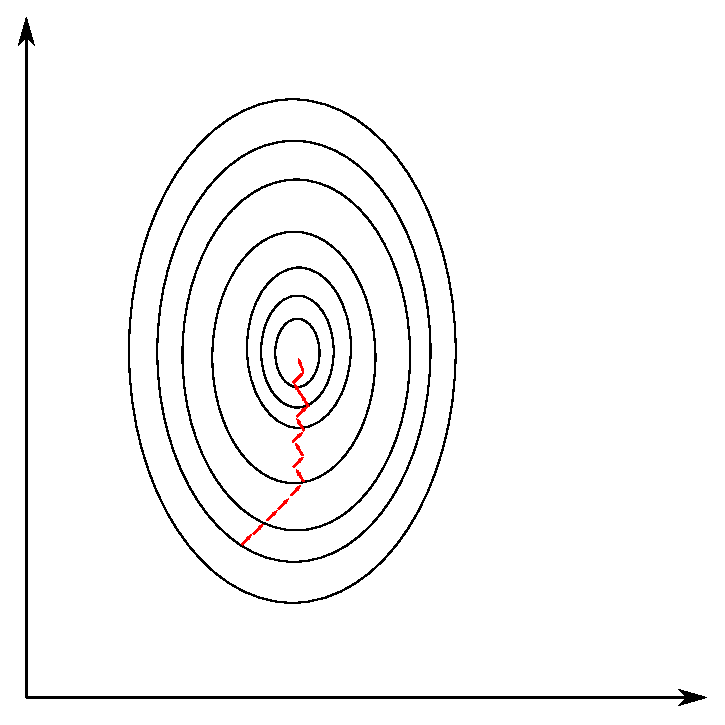
\includegraphics[width=0.5\textwidth]{FeatureScalingNoScale}
  \caption{With the axis $\Theta_1$ and $\Theta_2$}\label{fig:app:FeatureScalingNoScale}
\end{figure}

He it is use full to scale the features, so for our examples with $x_1, x_2$ we would scale them like $x_1 = \frac{\text{size(feet)}^2}{2000}$ and $x_2=\frac{\text{number of bedrooms}}{5}$. This will result in what we see in figure \ref{fig:app:FeatureScalingScale}

\begin{figure}[H]
  \centering
  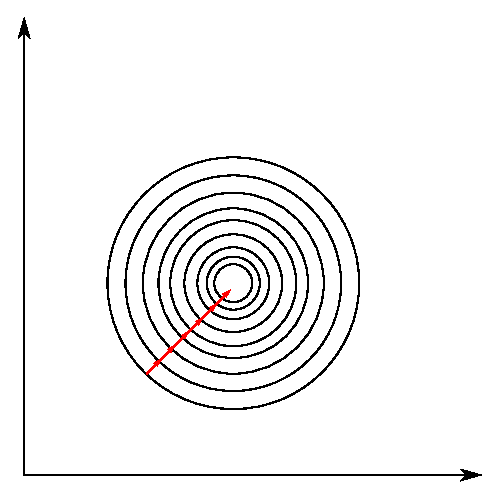
\includegraphics[width=0.5\textwidth]{FeatureScalingScale}
  \caption{With the axis $\Theta_1$ and $\Theta_2$}\label{fig:app:FeatureScalingScale}
\end{figure}

where we in figure \ref{fig:app:FeatureScalingScale} can see that we can find a much faster path to the global minimum.
In this example we end with both features $0\leq x_i \leq 1$ for $i=1,2$.

\subsection{Mean normalization}

Replace $x_i$ with $x_i - \mu_i$ to make features have approximately zero mean -- Do not apply to $x_0=1$.

\subsection{Choose the learning}

Look Lecture 4.4

\section{Choosing optimal variable}

When computing

\begin{equation}\label{fig:app:normalequationexample}
  (\matr{X}^T\matr{X})^{-1}\matr{X}^Ty
\end{equation}

What if $\matr{X}^T\matr{X}$ is non-invertible? (singular/degenrate). If it is non-invertible, there are two curses, the first one is if we have redundant features.
This is if we have $x_1 = \text{(feet)}^2x_2$ then we have linearly dependency.
The second reason is if we have too many features, $m\leq n$, then we have to delete some features or use regularization.

\section{Regularization}

When we apply machine learning problem, we can get overfitting problems, that can make our machineling learning algorithm to perform poorly.

\begin{figure}[H]
  \centering
  \begin{subfigure}{0.33\textwidth}
    \centering
    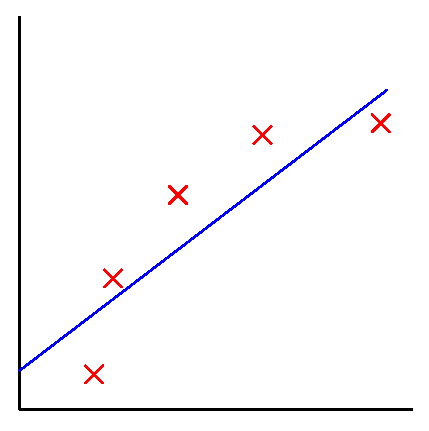
\includegraphics[width=.7\linewidth]{underfitexample.eps}
    \caption{This is an example of underfit and high bias, where our function looks like $\theta_0 + \theta_1x$}
    \label{fig:app:underfittingexample}
  \end{subfigure}
  \begin{subfigure}{0.33\textwidth}
    \centering
    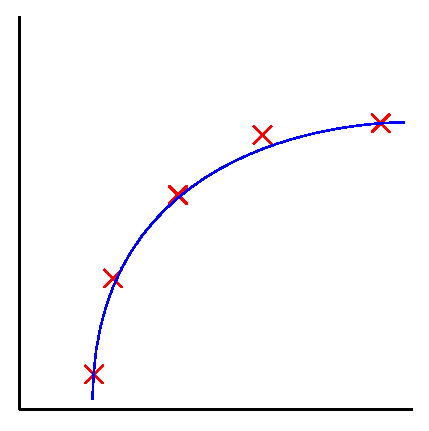
\includegraphics[width=.7\linewidth]{perfectfitexample.eps}
    \caption{This is an example of a good fit $\theta_0 + \theta_1x + \theta_2x^2$}
    \label{fig:app:perfectfitexample}
  \end{subfigure}
  \begin{subfigure}{0.33\textwidth}
    \centering
    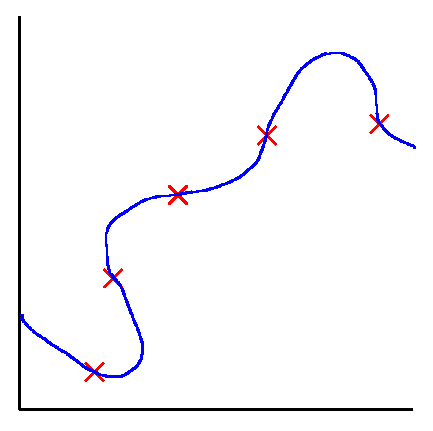
\includegraphics[width=.7\linewidth]{overfitexample.eps}
    \caption{This is an example of a overfitting, where we have a high variance $\theta_0 + \theta_1x + \theta_2x^2 + \theta_3x^3 + \theta_4x^4$}
    \label{fig:app:overfittingexample}
  \end{subfigure}
  \caption{Example of underfitting, overfitting and a good fit}
\end{figure}

With overfitting, we have too many features, the learned hypothesis may fit the training set very well, where our cost function

\[
  J(\theta) = \frac{1}{2m}\left(\sum_{i=1}^{m}(h_\theta(x^{(i)})-y^{(i)}\right)^2 \approx 0
\]

or as written in \cite{bishop2006pattern}

\[
  E(\matr{w}) = \frac{1}{2}\sum_{n=1}^{N}\{t_n - \matr{w}^T\phi(\matr{x}_n)\}^2
\]

but it fails to generalize to new examples.

A way to address overfitting is to regularize our data. We end up keeping all the features, but reduce the magnitude/values of parameters $\theta$ or as in \cite{bishop2006pattern} $\matr{w}$. This works well when we have a lot of features, each of which contributes a bit to predicting $y$

If we look at our figure \ref{fig:app:perfectfitexample} and \ref{fig:app:overfittingexample}, then suppose that we penalize and make $\theta_3,\theta_4$ really small.

If we look at our cost function

\[
  \min_\theta \frac{1}{2m}(\sum_{i=1}^{m}(h_\theta(x^{(i)})-y^{(i)})^2 + \textcolor[rgb]{0.00,0.09,0.92}{1000\theta^2_3} + \textcolor[rgb]{0.00,0.09,0.92}{1000\theta^2_4}
\]

this new cost function we will end up with $\theta_3 \approx 0$ and $\theta_4 \approx 0$ and we will end up with $\theta_0 + \theta_1x + \theta_2x^2$, which is our quadratic function as seen in figure \ref{fig:app:overfitexampleregularized}.

\begin{figure}[H]
  \centering
  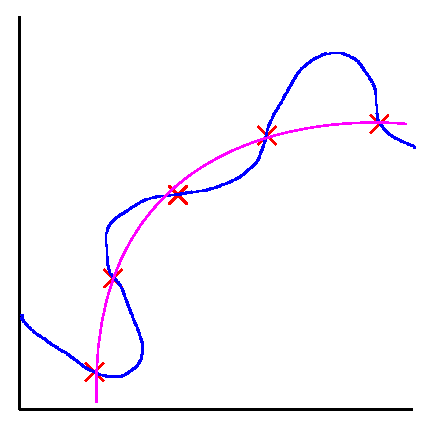
\includegraphics[width=0.4\textwidth]{overfitexampleregularized}
  \caption{Our function is a better fit now, since it has been regularized. The new function is quadratic}\label{fig:app:overfitexampleregularized}
\end{figure}

So the main intuition of how regularization works is, that if we have small values for parameters $\theta_0, \theta_1, ... ,\theta_n$, vi have a "simpler" hypothesis and is less prone to overfitting.
With our housing example, we could have features $x_1, x_2, ... , x_100$ and parameters $\theta_0, \theta_1, ... , \theta_{100}$ and don't know which parameters to "shrink". If we return to our cost function $J(\theta)$, then we add an extra term to it, e.g.

\[
  J(\theta) = \frac{1}{2m}(\sum_{i=1}^{m}(h_\theta(x^{(i)})-y^{(i)})^2 + \lambda \sum_{i=1}^{n} \theta_j^2
\]

or written as

\[
  J(\theta) = \frac{1}{2m}(\sum_{i=1}^{m}(h_\theta(x^{(i)})-y^{(i)})^2 + \lambda \matr{\theta}^T\matr{\theta}
\]

where all of my parameters $\theta_1, \theta_2, ... , \theta_{100}$ will get penalized. The lambda is our regularization parameter, it controls a tradeoff between two goals, where the first goal is that we want fit the training set well and the second goal is to keep the parameters small. $\lambda$ controls this tradeoff to avoid overfitting.

\section{Neural Networks}

Neurons bla bla bla.

\begin{figure}[H]
  \centering
  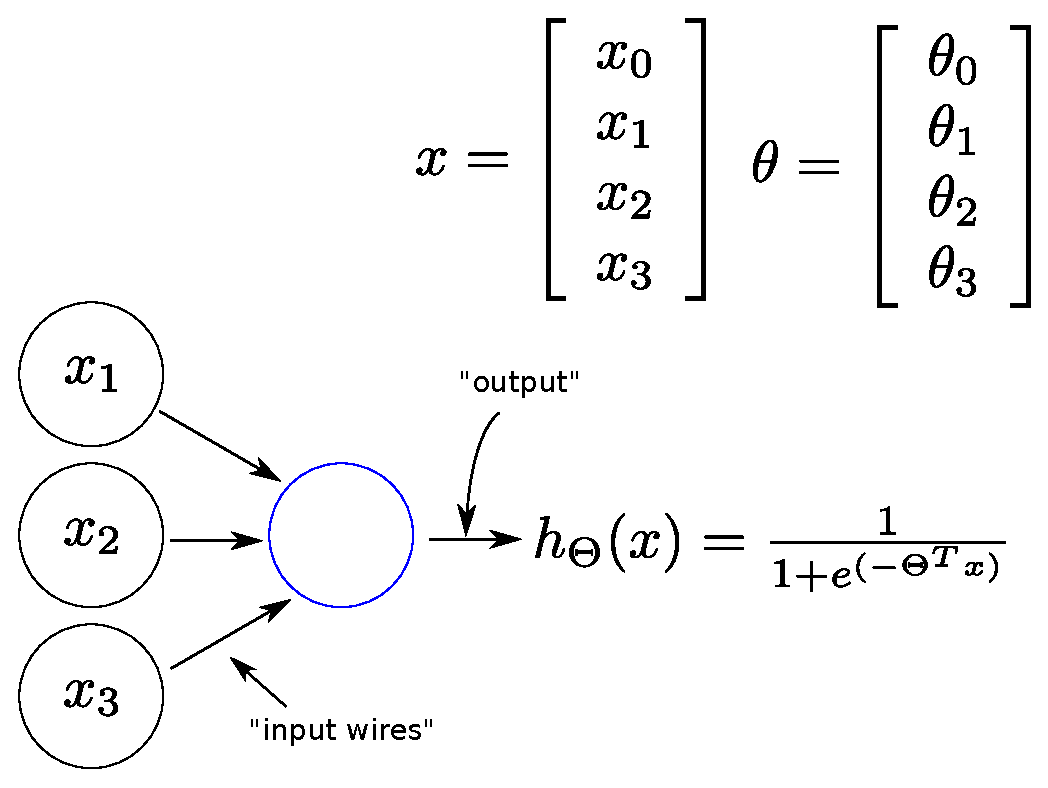
\includegraphics[width=0.7\textwidth]{simpleNNmodel.eps}
  \caption{Simple Neuron model: Logistic unit}\label{fig:app:simpleNNmodel}
\end{figure}

When drawning a neuron network, it is normal to draw the first 3 neurons, and the bias

\begin{figure}[H]
  \centering
  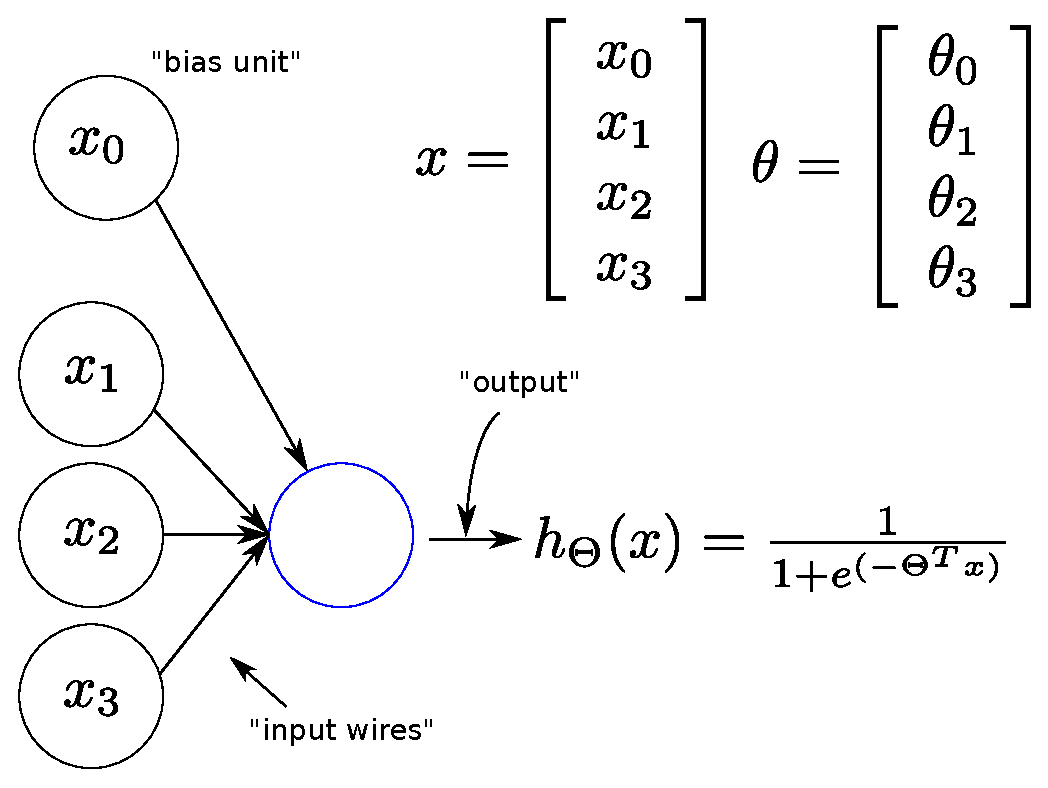
\includegraphics[width=0.7\textwidth]{simpleNNmodelbias.eps}
  \caption{Simple Neuron model: Logistic unit}\label{fig:app:simpleNNmodelbias}
\end{figure}

\begin{figure}[H]
  \centering
  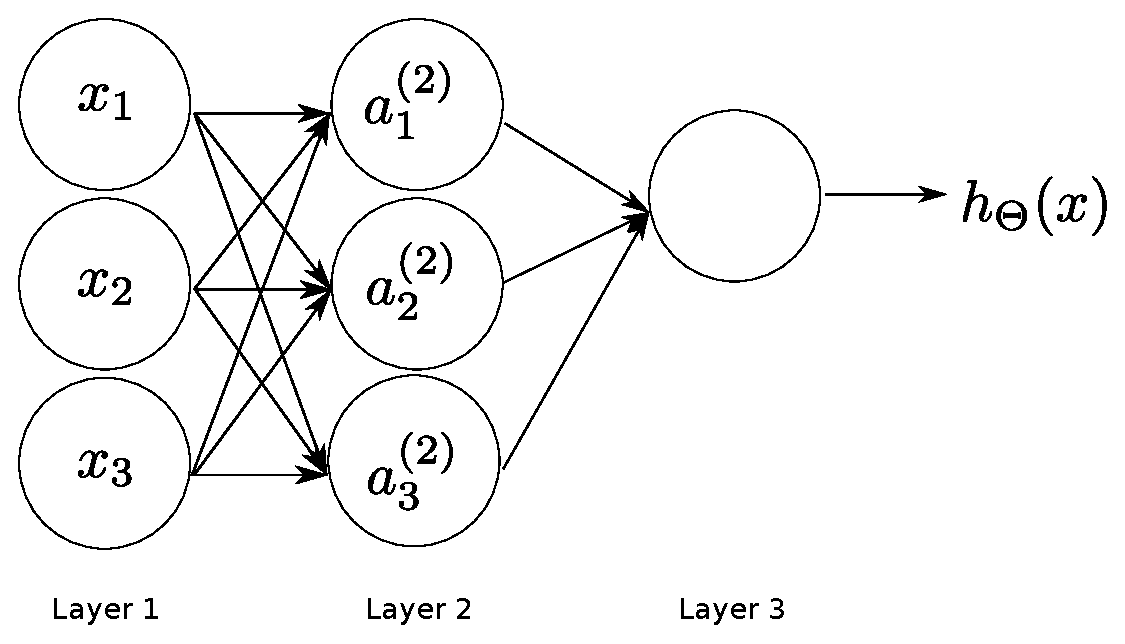
\includegraphics[width=0.7\textwidth]{neuralNetwork.eps}
  \caption{Simple Neuron model: Logistic unit}\label{fig:app:neuralNetwork}
\end{figure}

\begin{figure}[H]
  \centering
  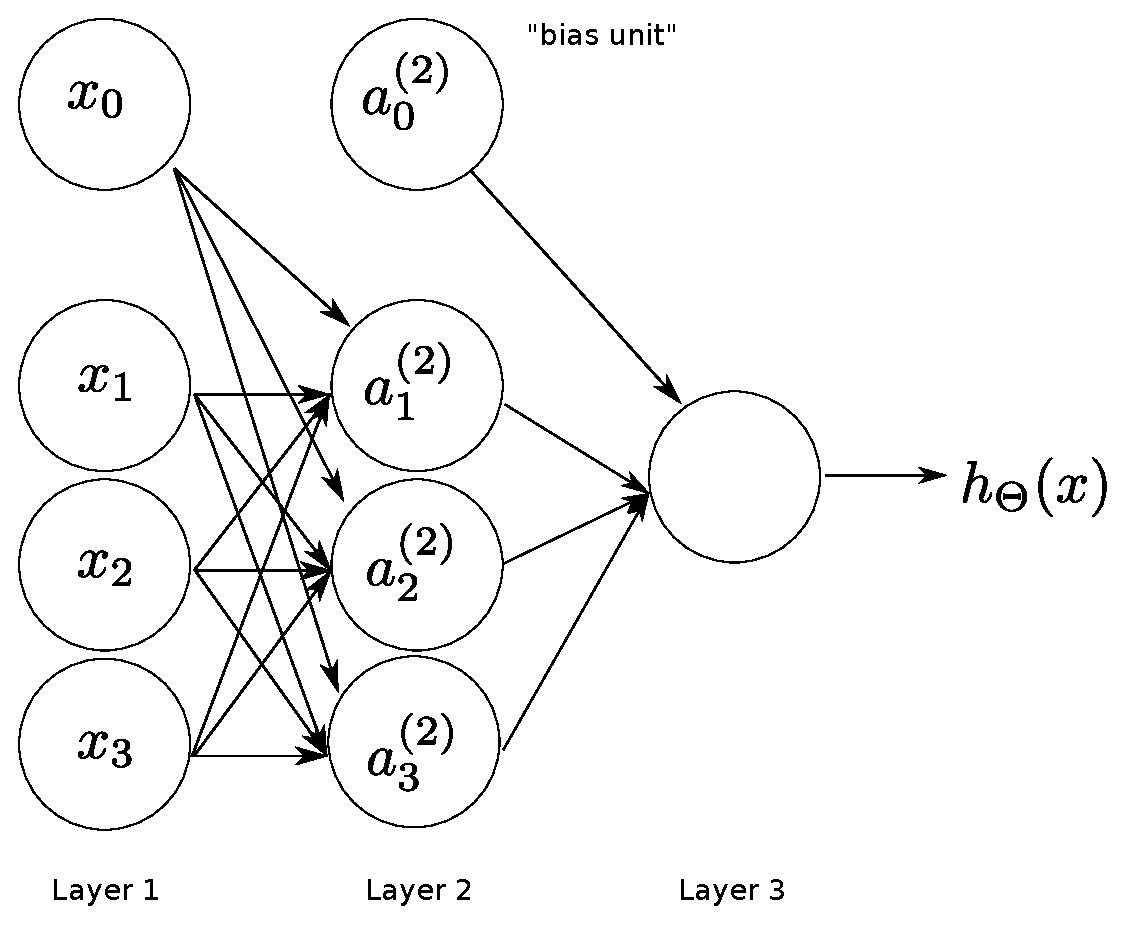
\includegraphics[width=0.7\textwidth]{neuralNetworkbias}
  \caption{Simple Neuron model: Logistic unit}\label{fig:app:neuralNetworkbias}
\end{figure}

So we denote the activation of unit \textit{i} in layer \textit{j} as $a_i^{(j)}$ and $\Theta^{(j)}$ is denoting the matrix of weigths controlling function mapping from layer \textit{j} to layer \textit{j}+1.

So from figure \ref{fig:app:neuralNetworkbias} the formulas will be defined as

\begin{align}\label{fig:app:activationfunctiontoneuralnetwork}
    a^{(2)}_1 =& g(\Theta^{(1)}_{10}x_0 + \Theta^{(1)}_{11}x_2 + \Theta^{(1)}_{12}x_2 + \Theta^{(1)}_{13}x_3) \\
    a^{(2)}_2 =& g(\Theta^{(1)}_{20}x_0 + \Theta^{(1)}_{21}x_2 + \Theta^{(1)}_{22}x_2 + \Theta^{(1)}_{23}x_3) \\
    a^{(2)}_3 =& g(\Theta^{(1)}_{30}x_0 + \Theta^{(1)}_{31}x_2 + \Theta^{(1)}_{32}x_2 + \Theta^{(1)}_{33}x_3)
\end{align}

where g is the activation function and the \textit{a}'s are the hidden units, while the \textit{x}'s are the input units. This makes the output unit to be

\begin{equation}
  h_\Theta(x) = a_1^{(3)} = g(\Theta^{(1)}_{10}a^{(2)}_0 + \Theta^{(1)}_{11}a^{(2)}_1 + \Theta^{(1)}_{12}a^{(2)}_2 + \Theta^{(1)}_{13}a^{(2)}_3)
\end{equation}

If the network has $s_j$ units in layer \textit{j}, $s_{j+1}$ units in layer \textit{j} + 1 then $\Theta^{(j)}$ wil be of dimension $s_{j+1} \times (s_j + 1)$

To make our notation easier, we will from now on denote $g(\Theta^{(1)}_{10}x_0 + \Theta^{(1)}_{11}x_2 + \Theta^{(1)}_{12}x_2 + \Theta^{(1)}_{13}x_3) = z_1^{(2)}$ and the next as $z_2^{(2)}$ and the last as $z_3^{(2)}$, so we will be able to rewrite equation \ref{fig:app:activationfunctiontoneuralnetwork} as

\begin{align}\label{fig:app:activationfunctiontoneuralnetworkrewritten}
    a^{(2)}_1 =& g(z_1^{(2)}) \\
    a^{(2)}_2 =& g(z_2^{(2)}) \\
    a^{(2)}_3 =& g(z_3^{(2)})
\end{align}

and lastly as

\begin{equation}
  h_\Theta(x) = a_1^{(3)} = g(z_1^{(3)})
\end{equation}

8.5, 8.6 for AND/OR examples for NN.

